%\documentclass{beamer}
%\usepackage{minijs}
%\usepackage{here}
%\mode<presentation>{
%  \usetheme{Antibes}
%  \usecolortheme{beaver}
%  \setbeamercovered{transparent}
%}
\documentclass[13pt,dvipdfmx]{beamer}
\usepackage[english]{babel}
% pdfの栞の字化けを防ぐ
\AtBeginDvi{\special{pdf:tounicode EUC-UCS2}}
% テーマ
\usetheme{CambridgeUS}
\usepackage{caption}
\setbeamertemplate{navigation symbols}{} 
\usepackage{graphicx}
\usepackage{amsmath}
\usepackage{amssymb}
\usepackage{txfonts}
\usepackage{colortbl}
\usepackage{svg}
\usepackage{pdfpages}
\renewcommand{\familydefault}{\sfdefault}
\renewcommand{\kanjifamilydefault}{\gtdefault}
\setbeamerfont{title}{size=\large,series=\bfseries}
\setbeamerfont{frametitle}{size=\large,series=\bfseries}
\setbeamertemplate{frametitle}[default][center]
\usefonttheme{professionalfonts} 

%1ページめ
\title{クラスタサイズ調整変数を導入したクラスタリング手法の評価}
\author{池辺 颯一}
\institute{芝浦工業大学 工学部 通信工学科}
\date{2018年12月12日}

\begin{document}
\begin{frame}\frametitle{}
 \titlepage
\end{frame}

\begin{frame}\frametitle{概要・背景}
\begin{itemize}
 \item 情報化社会の発展によりデータが複雑かつ膨大に
 \item ビッグデータを人の手で分類するのは難しい
 \item それらのデータを自動的に分類するクラスタリングに着目
\end{itemize}
\vspace{5mm}
\begin{figure}[htbp]
 \begin{minipage}{0.4\hsize}
  \begin{center}
   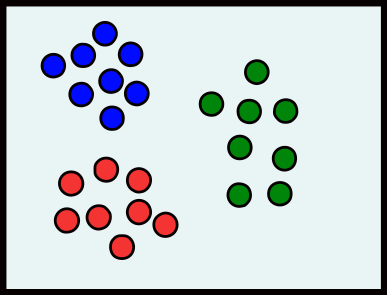
\includegraphics[width=40mm]{before_clustering.png}
  \end{center}
  \captionsetup{labelformat=empty,labelsep=none}
  \caption{クラスタリング前}
  \label{fig:one}
 \end{minipage}
\hspace{1cm}
 \begin{minipage}{0.4\hsize}
  \begin{center}
   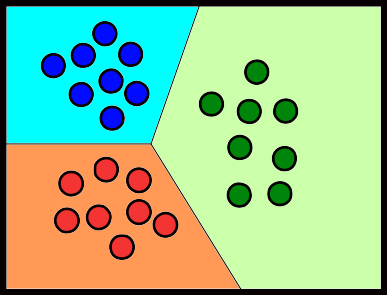
\includegraphics[width=40mm]{after_clustering.png}
  \end{center}
  \captionsetup{labelformat=empty,labelsep=none}
  \caption{クラスタリング後}
  \label{fig:two}
 \end{minipage}
\end{figure}
\end{frame}

\begin{frame}\frametitle{目的・目標}
\begin{block}{目的}
\begin{itemize}
\item クラスタリング手法の1つであるFussy c-meansの中からよりよい手法を発見する
\end{itemize}
\end{block}
\vspace{4mm}
\begin{block}{目標}
  \begin{itemize}
  \item クラスタサイズ調整変数を導入した最適化問題の中から最も精度が高いものを発見する
\end{itemize}
\end{block}
\end{frame}

\begin{frame}\frametitle{実験対象}
 \begin{block}{提案手法}
   \begin{itemize}
    \item eFCMA
    \item qFCMA
    \item sFCMA
   \end{itemize}
 \end{block}
\end{frame}

\begin{frame}\frametitle{クラスタリングの最適化問題}
  \begin{block}{eFCMA}
  \quad$\underset{u,v,\alpha}{\text{minimize}}$
    $\sum_{i=1}^C\sum_{k=1}^Nu_{i,k}||x_k-v_i||_2^2+\lambda^{-1}\sum_{i=1}^C\sum_{k=1}^Nu_{i,k}\log\Bigl(\frac{u_{i,k}}{\alpha_{i}}\Bigl)$
    \qquad{\text{subject to}}$\sum_{i=1}^Cu_{i,k}=1$\;,\;$\sum_{i=1}^C\alpha_{i}=1$\;and\;$u_{i,k}\in[0,1]$\quad$m>1$
  \end{block}
  \begin{center}
\begin{tabular}{c|c||c|c} \hline
	{$N$}&データ数&{$x_k$}&データ数 \\ \hline
	{$C$}&クラスタ数&{$v_i$}&クラスタ中心\\ \hline
	{$\lambda$}&ファジィ化パラメータ&{$u_{i,k}$}&帰属度 \\ \hline
	{$\alpha_i$}&クラスタサイズ調整変数\\ \hline
\end{tabular}
\end{center}
\end{frame}

\begin{frame}\frametitle{クラスタリングの最適化問題}
  \begin{block}{qFCMA}
    \quad$\underset{u,v,\alpha}{\text{minimize}}$
    $\sum_{i=1}^C\sum_{k=1}^N(\alpha_{i})^{1-m}(u_{i,k})^m||x_k-v_i||_2^2$\\
    \qquad\qquad\qquad\qquad$+\frac{\lambda^{-1}}{m-1}\sum_{i=1}^C\sum_{k=1}^N(\alpha_{i})^{1-m}(u_{i,k})^m$
    \qquad{\text{subject to}}$\sum_{i=1}^Cu_{i,k}=1$\;,\;$\sum_{i=1}^C\alpha_{i}=1$\;and\;$u_{i,k}\in[0,1]$\quad$m>1$
  \end{block}
  \begin{center}
\begin{tabular}{c|c||c|c} \hline
	{$N$}&データ数&{$x_k$}&データ数 \\ \hline
	{$C$}&クラスタ数&{$v_i$}&クラスタ中心\\ \hline
	{$\lambda,m$}&ファジィ化パラメータ&{$u_{i,k}$}&帰属度 \\ \hline
	{$\alpha_i$}&クラスタサイズ調整変数\\ \hline
\end{tabular}
\end{center}
\end{frame}

\begin{frame}\frametitle{クラスタリングの最適化問題}
  \begin{block}{sFCMA}
    \quad$\underset{u,v,\alpha}{\text{minimize}}$
    $\sum_{i=1}^C\sum_{k=1}^N(\alpha_{i})^{1-m}(u_{i,k})^m||x_k-v_i||_2^2$\\
    \qquad{\text{subject to}}$\sum_{i=1}^Cu_{i,k}=1$\;,\;$\sum_{i=1}^C\alpha_{i}=1$\;and\;$u_{i,k}\in[0,1]$\quad$m>1$
  \end{block}
  \begin{center}
\begin{tabular}{c|c||c|c} \hline
	{$N$}&データ数&{$x_k$}&データ数 \\ \hline
	{$C$}&クラスタ数&{$v_i$}&クラスタ中心\\ \hline
	{$m$}&ファジィ化パラメータ&{$u_{i,k}$}&帰属度 \\ \hline
	{$\alpha$}&クラスタサイズ調整変数\\ \hline
\end{tabular}
\end{center}
\end{frame}

\begin{frame}\frametitle{アルゴリズム}
\begin{block}{FCM(Fusssy c-means)}
\begin{enumerate}
 \item 初期クラスタ中心Vを与える
 \item Vから帰属度Uを更新する
 \item Vを更新する
 \item 収束条件を満たせば終了。満たさなければ2へ。
\end{enumerate}
\end{block}
\end{frame}

\begin{frame}\frametitle{実験方法}
\begin{center}
 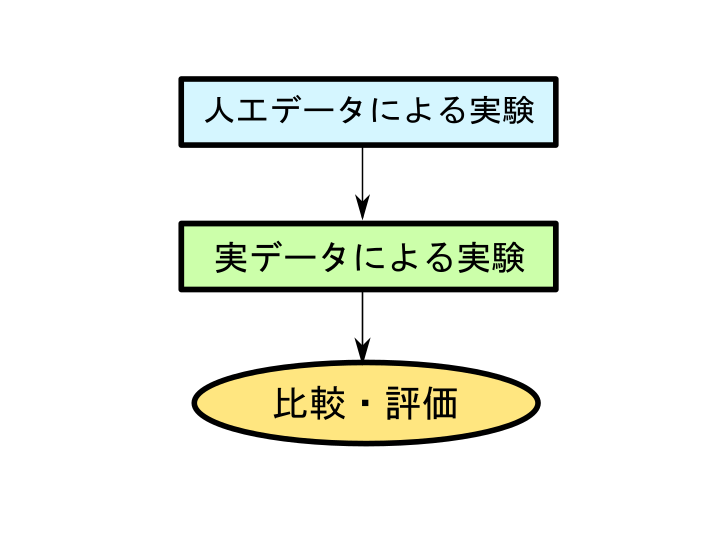
\includegraphics[width=100mm]{experiment_process.png}
\end{center}
\end{frame}

\begin{frame}\frametitle{評価方法}
\begin{block}{ARI (Adjusted Rand Index)}
\begin{itemize}
 \item -1から1までの範囲で精度評価を行う指標
 \item 1の時に完全一致で0の時にランダム
 \item ARIの値が高いほど高評価
\end{itemize}
\end{block}
\begin{center}
\end{center}
\end{frame}

\begin{frame}\frametitle{人工データ実験}
  \begin{block}{使用する人工データ}
    \begin{itemize}
    \item 平均値(-1, -1)標準偏差(0.5, 0.5)のガウスサンプリングで生成
    \item データ数: 100
    \item クラス数 : 2
    \end{itemize}
  \end{block}
\end{frame}

\begin{frame}\frametitle{実験結果:人工データ}
  \begin{block}{eFCMA}
   \begin{figure}[htbp]
    \begin{center}
    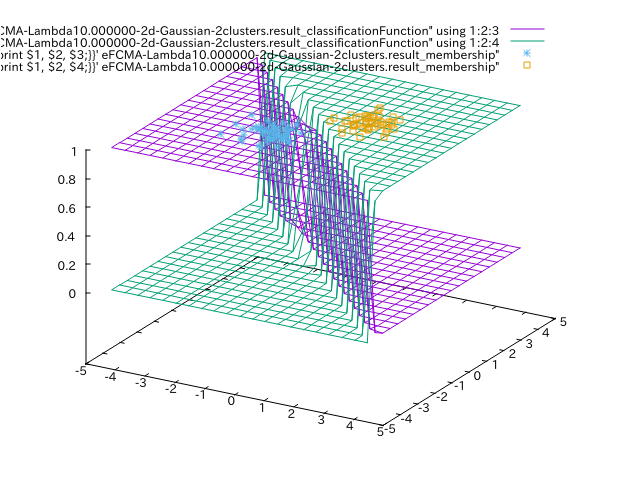
\includegraphics[height=60mm]{eFCMA-Lambda10.png}
   \end{center}
   \captionsetup{labelformat=empty,labelsep=none}
   \caption{$\lambda=10.0$}
  \end{figure}
 \end{block}
\end{frame}

\begin{frame}\frametitle{実験結果:人工データ}
  \begin{block}{sFCMA}
   \begin{figure}[htbp]
    \begin{center}
    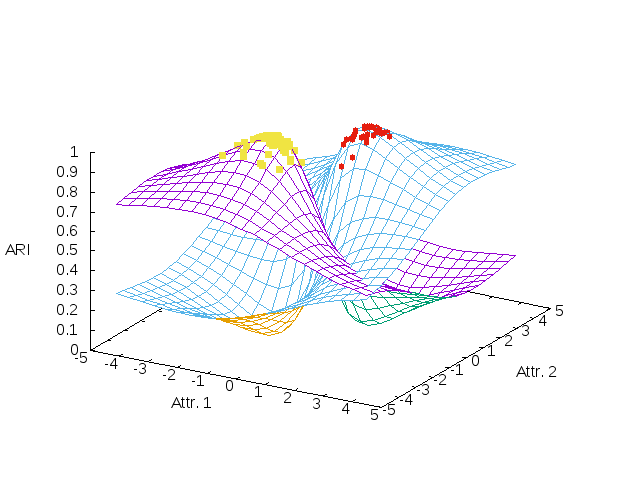
\includegraphics[height=60mm]{sFCMA-Em2.png}
   \end{center}
    \captionsetup{labelformat=empty,labelsep=none}
   \caption{$m=2.0$}
  \end{figure}
 \end{block}
\end{frame}


\begin{frame}\frametitle{実験結果:人工データ}
  \begin{block}{qFCMA}
  %\vspace{5mm}
   \begin{figure}[htbp]
 \begin{minipage}{0.32\hsize}
  \begin{center}
   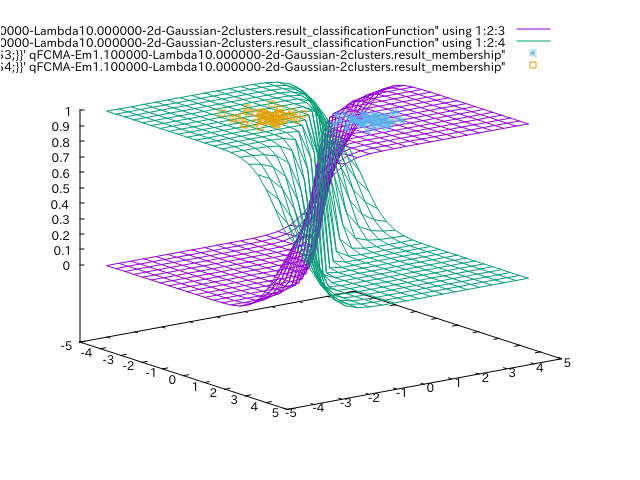
\includegraphics[width=32mm]{qFCMA-Em11-Lambda10.png}
  \end{center}
  \captionsetup{labelformat=empty,labelsep=none}
  \caption{$m=1.1, \lambda=10.0$}
  \label{fig:one}
 \end{minipage}
%\hspace{1cm}
 \begin{minipage}{0.32\hsize}
  \begin{center}
   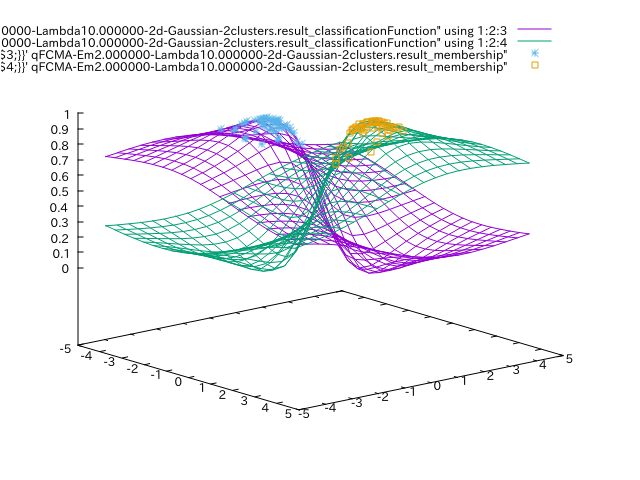
\includegraphics[width=32mm]{qFCMA-Em2-Lambda10.png}
  \end{center}
  \captionsetup{labelformat=empty,labelsep=none}
  \caption{$m=2.0, \lambda=10.0$}
  \label{fig:two}
 \end{minipage}
 %\hspace{1cm}
 \begin{minipage}{0.32\hsize}
  \begin{center}
   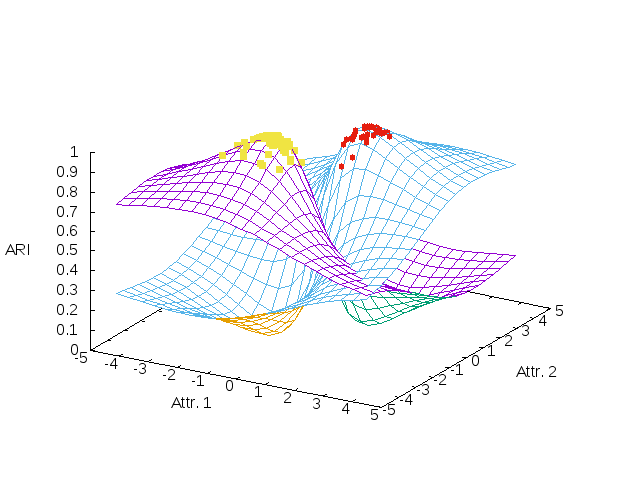
\includegraphics[width=32mm]{qFCMA-Em2-Lambda10000.png}
  \end{center}
  \captionsetup{labelformat=empty,labelsep=none}
  \caption{$m=2.0, \lambda=10000$}
  \label{fig:three}
 \end{minipage}
\end{figure}
 \end{block}
\end{frame}

\begin{frame}\frametitle{実データ実験}
  \begin{block}{User Knowledge Modeling Data Set}
    \begin{itemize}
    \item 被験者の勉強時間、試験結果など5属性を収録したデータ
    \item ソース : UCI  Machine Learning Repository
    \item 個体数 : 403
    \item クラス数 : 4(非常に低い、低い、中央、高い)
    \end{itemize}
  \end{block}
\end{frame}


\begin{frame}\frametitle{実験条件}
\begin{block}{eFCMA}
  パラメータ$\lambda$を6.0から0.1刻みで10.0まで変化させた際のARIを導出
\end{block}
\begin{block}{qFCMA}
  \begin{itemize}
  \item パラメータ$\lambda$を10.0で固定し、パラメータmを2.0から0.1刻みで1.1まで変化させた際のARIを導出
  \item パラメータ$m$を2.0で固定し、パラメータ$\lambda$50.0から10刻みで200まで変化させた際のARIを導出
  \end{itemize}
\end{block}
\begin{block}{sFCMA}
  パラメータ$m$を3.0から0.1刻みで1.1まで変化させた際のARIを導出
\end{block}

\end{frame}

\begin{frame}\frametitle{実験結果:実データ}
  \begin{block}{eFCMA}
   \begin{figure}[htbp]
    \begin{center}
     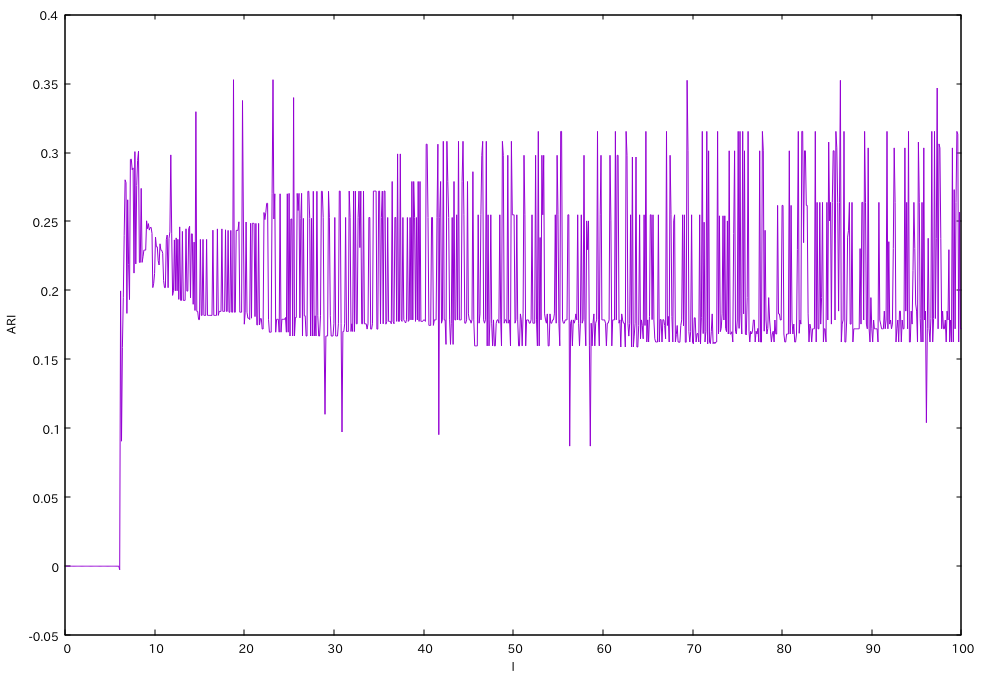
\includegraphics[height=60mm]{efcma_ARI.png}
   \end{center}
   \captionsetup{labelformat=empty,labelsep=none}
   \caption{最高ARI:0.309493}
  \end{figure}
 \end{block}
\end{frame}


\begin{frame}\frametitle{実験結果:実データ}
  \begin{block}{qFCMA}
   \begin{figure}[htbp]
    \begin{center}
    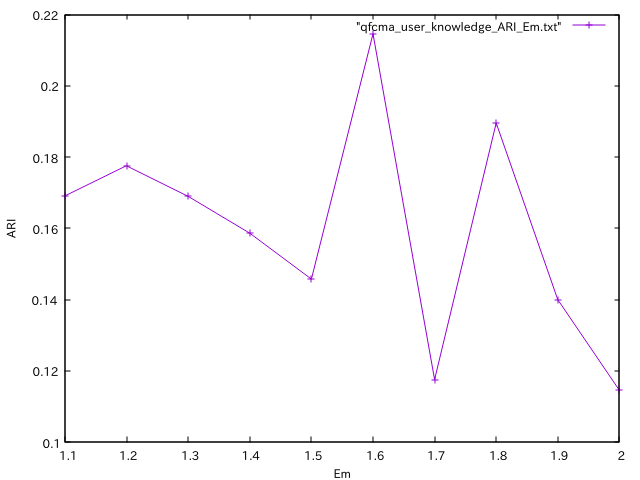
\includegraphics[height=60mm]{qfcma_ARI_Em.png}
   \end{center}
   \captionsetup{labelformat=empty,labelsep=none}
   \caption{$\lambda$=10.0  最高ARI:0.229751}
  \end{figure}
 \end{block}
\end{frame}

\begin{frame}\frametitle{実験結果:実データ}
  \begin{block}{qFCMA}
   \begin{figure}[htbp]
    \begin{center}
    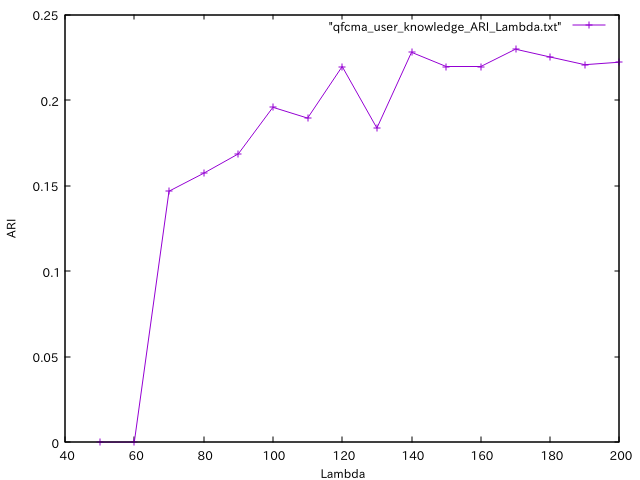
\includegraphics[height=60mm]{qfcma_ARI_Lambda.png}
   \end{center}
   \captionsetup{labelformat=empty,labelsep=none}
   \caption{m=2.0 最高ARI:0.214619}
  \end{figure}
 \end{block}
\end{frame}

\begin{frame}\frametitle{実験結果:実データ}
  \begin{block}{sFCMA}
   \begin{figure}[htbp]
    \begin{center}
    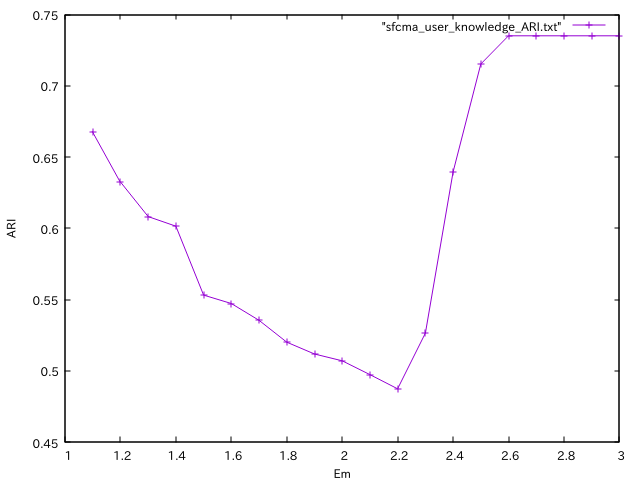
\includegraphics[height=60mm]{sfcma_ARI.png}
   \end{center}
   \captionsetup{labelformat=empty,labelsep=none}
   \caption{最高ARI:0.73515}
  \end{figure}
 \end{block}
\end{frame}

\begin{frame}\frametitle{実験結果}
\begin{block}{各手法の最高ARI}
\vspace{5mm}
  \begin{table}[htb]
   \begin{tabular}{ l | c }\hline
     eFCMA & 0.309493 \\ \hline  
     qFCMA & 0.222143\\  \hline
     sFCMA & 0.73515\\ \hline
   \end{tabular}
  \end{table}
  sFCMAが最も高評価となった
 \end{block}
\end{frame}

\begin{frame}\frametitle{考察・課題}
  \begin{block}{考察}
    \begin{itemize}
    \item sFCMAとeFCMA、qFCMAとの差は、エントロピー項の有無。
    \item エントロピー項を削除したことが計算結果に影響したと考えられる。
    \end{itemize}
    \end{block}
  \begin{block}{課題}
    \begin{itemize}
    \item 他の実データでも同様の傾向が現れるかどうかの検証。
    \item エントロピー項が影響する原因及び理由の調査。
    \end{itemize}
    \end{block}
\end{frame}

\begin{frame}\frametitle{まとめ}
  \begin{block}{目的}
    \begin{itemize}
    \item クラスタリング手法の1つであるFussy c-meansの中からより確実な手法を発見する
    \end{itemize}
  \end{block}
  \begin{block}{目標}
    \begin{itemize}
     \item クラスタサイズ調整変数を導入した最適化問題の中から最も精度が高いものを発見する
     \item C++プログラムの実行結果からクラスタリング精度を評価
    \end{itemize}
  \end{block}
  \begin{block}{実験結果}
    \begin{itemize}
    \item sFCMAが高評価となった
    \end{itemize}
  \end{block}
  \begin{block}{考察}
    \begin{itemize}
    \item エントロピー項を削除したことが計算結果に影響したと考えられる
    \end{itemize}
  \end{block}
\end{frame}

\begin{frame}\frametitle{補足:eFCMAの更新式}
   \begin{eqnarray*}
   &v_{i}& =\frac{\sum_{k=1}^Nu_{i,k}x_{k}}{\quad\sum_{k=1}^Nu_{i,k}},\\
   &u_{i,k}&=\frac{\pi_{i}\exp(-\lambda||x_k-v_i||_2^2)}{\sum_{j=1}^C\pi_{j}\exp(-\lambda||x_k-v_j||_2^2)},\\
   &\alpha_{i}&=\frac{\sum_{k=1}^Nu_{i,k}}{\quad N}.\\
   \end{eqnarray*}
\end{frame}

\begin{frame}\frametitle{補足:qFCMAの更新式}
  \begin{eqnarray*}
    &v_{i}&=\frac{\sum_{k=1}^N(u_{i,k})^mx_{k}}{\quad\sum_{k=1}^N(u_{i,k})^{m}},\quad\\
    &u_{i,k}&=\frac{\alpha_{i}(1+\lambda(1-m)||x_i-v_k||_2^2)^\frac{1}{1-m}}{\quad\sum_{j=1}^C\alpha_{j}(1+\lambda(1-m)||x_j-v_k||_2^2)^\frac{1}{1-m}},\\
    & \alpha_{i}&=\frac{1}{\sum_{j=1}^C\left(\sum_{k=1}^N\frac{(u_{j,k})^m(1-\lambda(1-m)d_{j,k})}{(u_i,k)^m(1-\lambda(1-m)d_{i,k})}\right)^{\frac{1}{m}}}.\\
      \end{eqnarray*}
\end{frame}

\begin{frame}\frametitle{補足:sFCMAの更新式}
  \begin{eqnarray*}
  &v_{i}&=\frac{\sum_{k=1}^N(u_{i,k})^mx_{k}}{\quad\sum_{k=1}^N(u_{i,k})^{m}},\\
  &u_{i,k}&=\frac{1}{\sum_{j=1}^c\frac{\alpha_{j}}{\alpha_{i}}\left(\frac{d_{j,k}}{d_{i,k}}\right)^\frac{1}{1-m}},\\
  &\alpha_{i}&=\frac{1}{\sum_{j=1}^C\left(\sum_{k=1}^N\frac{(u_{j,k})^md_{j,k}}{(u_{i,k})^md_{i,k}}\right)^{\frac{1}{m}}}.\\
  \end{eqnarray*}
\end{frame}

\end{document}
